% !TeX spellcheck = en_US
% !TeX root = notes.tex
\section{Combination Logic}
\subsection{Combinational Circuits}
Each output can be expressed as a function of $n$ input variables. Can write truth table also:
\begin{itemize}
	\item $n$ input columns
	\item $m$ output columns
	\item $2^n$ rows (i.e. possible input combination)
\end{itemize}

\begin{note}{Multiplexer (or Mux)}
	\begin{itemize}
		\item $2^n$ data inputs
		\item 1 output
		\item $n$ control (or \textbf{select}) inputs - that \textbf{select} one of the inputs to be ``sent'' or ``steered'' to the output	
	\end{itemize}
\end{note}

\begin{note}{Decoder}
	Converts $n$-bit input to a logic-1 on exactly one of $2^n$ outputs	
\end{note}

\subsection{Timing Diagram}
\begin{figure}[H]
	\begin{tikztimingtable}[timing/slope=0,timing/coldist=2pt,xscale=4,semithick]
		Input & LHL \\
		Output & HLH \\
		\extracode\makeatletter
		\begin{pgfonlayer}{background}
			\begin{scope}[gray,semitransparent,semithick]
				\horlines{}
				\vertlines{0,...,3}	
			\end{scope}
		\end{pgfonlayer}
	\end{tikztimingtable}
	\centering\caption{Timing Diagram of an inverter}
\end{figure}

There is a slight delay in logic timings in reality
\begin{figure}[H]
	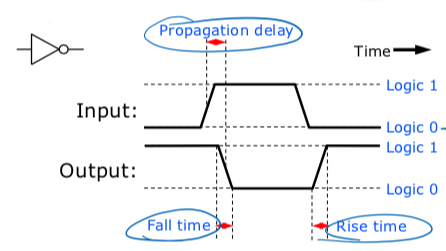
\includegraphics[width=0.8\linewidth]{timing}
	\centering\caption{Reality of Timing}
\end{figure}
\begin{description}
	\item[Propagation delay:] time for change in input to affect output
	\item[Fall time:] time taken for output to fall from 1 to 0
	\item[Rise time:] time for output to rise from 0 to 1	
\end{description}



